\SubProblem
{تابع کمکی برای اسپیس‌گذاری}
{
\begin{figure}[H]
    \centering
    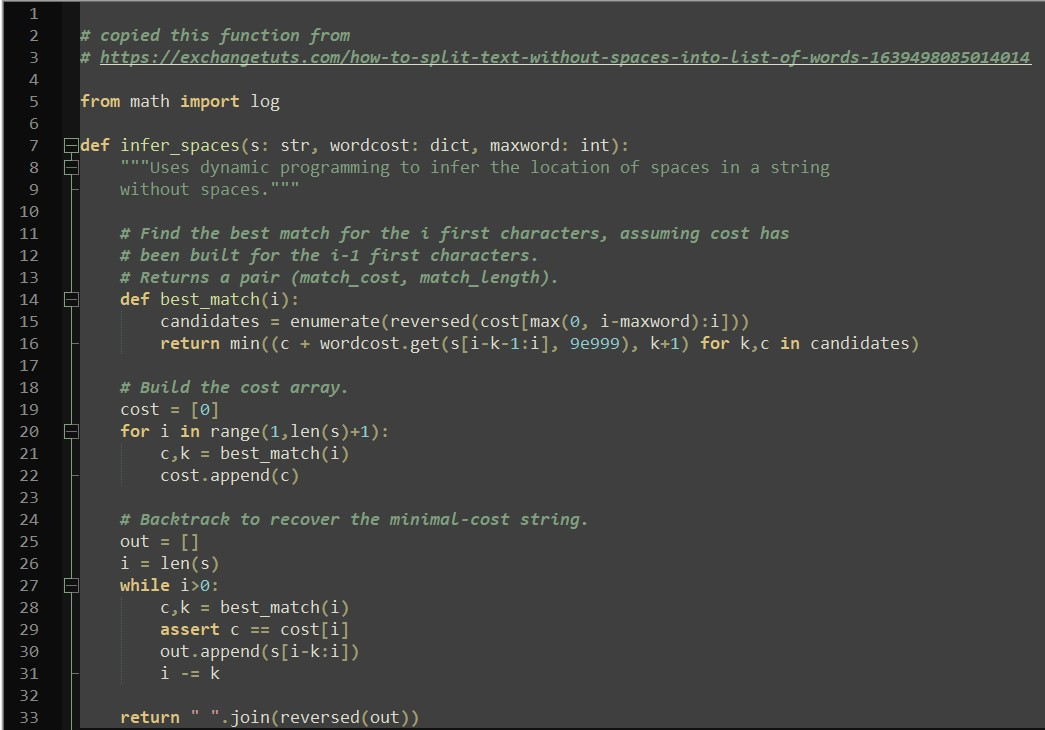
\includegraphics[width=15cm]{Images/F6.jpg}
    \label{fig:label}
    \caption{تابع کمکی برای اسپیس‌گذاری}
\end{figure}

این قسمت از یک اینترنت برداشته شده است و برای ایجاد فاصله در یک رشته بدون فاصله بکار می‌رود. لینک آن در قسمت منابع موجود است.

نحوه کارکرد آن به صورت برنامه‌ریزی پویا
\lr{(Dynamic Programming)}
است.
به صورتی که طول‌های مختلفی برای جداسازی کلمات استفاده می‌شود و در هر مرحله یک هزینه
\lr{(Cost)}
محاسبه می‌شود.
در نهایت بهترین نتیجه خروجی داده می‌شود.
}
